\documentclass[12pt]{article}
\setlength\parindent{0pt}
\usepackage{graphicx}
\usepackage{pdflscape}

\begin{document}

Maps are one of the core visualization tools of Superphy and provide users with an interactive interface for obtaining and searching genomes with geospatial meta-information. Superphy has leveraged Google Maps along with their companion Javascript library, Google Maps API (V3), to provide a scalable visual interface for thousands of genomes to the user. Maps are ubiquitous throughout the application and have been designed in different flavours to enhance the various analysis tools the platform has to offer.

\section{Design and Performance}

Genomes with available isolation location meta-data are geocoded for their latitude and longitude and  are displayed on the maps as circular markers. Currently, there are hundreds to thousands of genomes with, sometimes overlapping, geospatial information in Superphy's database. Simply rendering each of the genome locations on the map can lead to a severe bottleneck in browser performance. Moreover, the utility as a visualization tool is degraded as map markers crowd the view port and become difficult to distinguish from one another.\\

To address these issues, we implemented marker clustering. Locations that fall within a certain defined distance from each other are clustered together into a single marker rendered at the geometric center of the cluster, and a count of the number of clustered locations is shown on the marker icon. As the user zooms in on the map the number of markers to display is reduced and individual locations re-materialize as single markers. A counter-effect occurs as the user zooms out of the map. 

Some genomes have identical isolation locations, therefore, markers for these genomes render at exactly the same spot on the map. Discerning genomes, at these locations, directly on the map is not currently feasible. As a result, maps are accompanied by a dynamic and sortable table of genome names that are, as a default setting, sorted by location. As users zoom in and out and pan across the maps, the table changes to show only those genomes currently in the map view port. We have also made isolation locations for each genome available for download in a tab delimited text file.

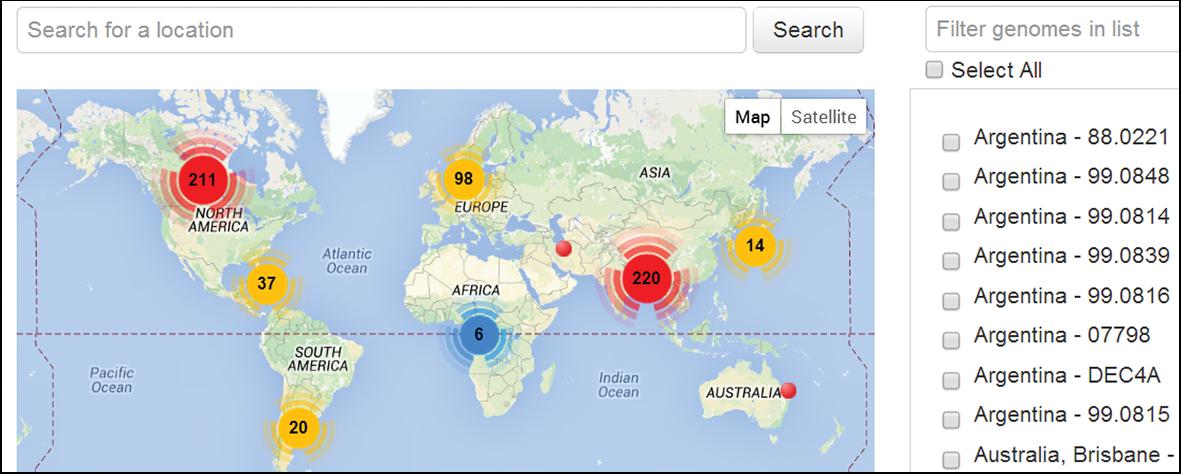
\includegraphics[scale=0.35]{../manuscript_images/map.png}

\section{Maps in Search}

Maps are highly integrated with Superphy's genome search and filtering controls.

\section{Maps in Genome Information}

Maps are used to highlight geospatial information about genomes.

\section{Maps in Geospatial-Phylogeny Information}

As an example genomes have been filtered to show only those isolated from Bovine in the the United States.

\pagebreak

\begin{landscape}
\includegraphics[scale=0.33]{../manuscript_images/geophy.png}
\end{landscape}


\end{document}